\documentclass[12pt]{article}

\usepackage[utf8]{inputenc}    
\usepackage[T1]{fontenc}
\usepackage[francais]{babel}
\usepackage{amsmath}
\usepackage{amssymb}
\usepackage{mathrsfs}
\usepackage{graphicx}


\begin{document}
 
\title{Chifoumi - Cahier des charges}
\author{M. Duprey \and M. Grimal \and E.Jeanmougin \and C. Leroux}
 
 
 \maketitle
 
 \newpage
 \tableofcontents
\newpage

\section{Règles du jeu}

\begin{itemize}

 \item C'est un jeu fait pour deux joueurs.
 \item Ce jeu se déroule sur un plateau (une grille de 7*7 cases) en forme de "+".
 \item On dispose sur ce plateau de pions ronds pouvant representer:
 \begin{itemize}
    \item[\textbullet] un puit
    \item[\textbullet] une pierre
    \item[\textbullet] une feuille
    \item[\textbullet] une paire de ciseaux
 \end{itemize}
\item Les pions se déplacent d'une case horizontalement, verticalement ou diagonalement.
\item Les déplacements autorisés sont les suivants:
\begin{itemize}
  \item[\textbullet]Déplacement d'un pion sur une case vide
  \item[\textbullet]Déplacement d'un pion sur un pion de sa propre couleur (empilement)
  \item[\textbullet]Déplacement d'un pion sur un pion de l'adversaire pouvant être pris
\end{itemize}
\item Les déplacements invalides sont :
\begin{itemize}
 \item[\textbullet] tout déplacement sortant du plateau 
 \item[\textbullet] tout déplacement sur un pion adverse ne pouvant être pris
\end{itemize}
  \item Les règles pour les prises des pions adverses sont les suivantes:
\begin{itemize}
  \item[\textbullet]Le puit prends la pierre et les ciseaux
  \item[\textbullet]La feuille prend le puit et la pierre
  \item[\textbullet]la pierre prend les ciseaux
  \item[\textbullet]Les ciseaux prennent la feuille
\end{itemize}
\item A chaque début de partie le plateau est initialisé de la façcon suivante:
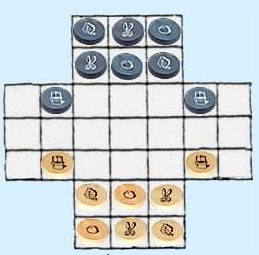
\includegraphics[width=0.5\textwidth]{images/init.png}
\item Lorqu'un qu'un pion est pris, il est alors retiré du plateau. Si ce pion était au sommet d'une pile, la totalité de la pile est alors retirée du plateau. 
\item Le nombre de points marqué par un joueur correspond au nombre de pions qu'il a pris à son adversaire.
\item La partie se termine lorsqu'un des joueurs n'a plus de pions ou lorsqu'il ne reste plus qu'une sorte de pions sur le plateau.
\item Le joueur gagnant est celui qui a marqué le plus de points. En cas d'égalité, le joueur qui a commencé perd.
\item Le joueur garde la main tant qu'il n'a pas fourni un déplacement valide
\end{itemize}

\section{Déroulement du programme}
 \begin{itemize}
 \item Au lancement de l'application, le programme
 \begin{itemize}
  \item[\textbullet] crée la grille
  \item[\textbullet] place les pions
  \item[\textbullet] crée et initialise les deux joueurs
 \end{itemize}
 \item En phase de jeu, le programme
 \begin{itemize}
  \item[\textbullet] présente à l'utilisateur l'état du jeu, le joueur ayant la main ou ayant gagné si la partie est finie et l'état de la grille (placement des pions)
  \item[\textbullet] fournit à l'utilisateur le moyen de désigner la nouvelle case et la précédente
  \end{itemize}
 
  \item affiche une alarme si le déplacement n'est pas valide, sinon change de joueur
  \item actualise ces informations jusqu'à la fin du jeu
 \end{itemize}
\section{version 1 : affichage en console}
\begin{itemize}
 \item Lors de cette version, chaque colonne est identifiée par un chiffre et chaque ligne par une lettre.
 \item Le joueur identifie donc la case de départ ainsi que la case d'arrivée par ses coordonnées (lettre,chiffre)
 \item Sur le plateau, on identifie un pion par un chiffre (taille de la pile) suivi d'une lettre (nature du sommet de la pile)
 \begin{itemize}
  \item[\textbullet] f : feuille
  \item[\textbullet] r : rock (pierre)
  \item[\textbullet] p : puit
  \item[\textbullet] c : ciseaux
 \end{itemize}
\end{itemize}
\centering{
  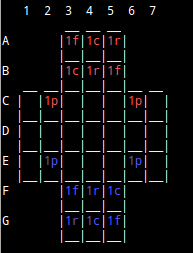
\includegraphics[width=5cm]{images/plateau.png}
  }
\section{version 2 : version graphique}
\begin{itemize}
 \item Lors de cette version, le plateau sera plus ressemblant à celui du jeu de société
 \item Cette fois, l'utilisateur interagira avec le plateau directement en cliquant sur les cases 
 \item Lorsqu'une case contenant un pion est selectionnée, les cases où le pion peut se déplacé sont affichées en surbrillance
 \item Sur le plateau, le nombre de pions empilés pourra être compté par le joueurs et chaque pion est identifié par un dessin
\end{itemize}

\section{version 3 : mode réseau}

Cette version reprend la version graphique précédente en permettant à deux joueurs de jouer l'un contre l'autre depuis deux ordinateurs différents par le biais du réseau.
 
\end{document}
